% !TEX TS-program = xelatex
% !BIB program = bibtex
% !TeX spellcheck = ru_RU

\documentclass{beamer}
%Для защит онлайн лучше использовать разрешение 16x9
%\documentclass[aspectratio=169]{beamer}

% !TeX spellcheck = ru_RU
% !TEX root = vkr.tex
% Опциональные добавления используемых пакетов. Вполне может быть, что они вам не понадобятся, но в шаблоне приведены примеры их использования.
\usepackage{tikz} % Мощный пакет для создание рисунков, однако может очень сильно замедлять компиляцию
\usetikzlibrary{decorations.pathreplacing,calc,shapes,positioning,tikzmark}

% Библиотека для TikZ, которая генерирует отдельные файлы для каждого рисунка
% Позволяет ускорить компиляцию, однако имеет свои ограничения
% Например, ломает пример выделения кода в листинге из шаблона
% \usetikzlibrary{external}
% \tikzexternalize[prefix=figures/]

\newcounter{tmkcount}

\tikzset{
  use tikzmark/.style={
    remember picture,
    overlay,
    execute at end picture={
      \stepcounter{tmkcount}
    },
  },
  tikzmark suffix={-\thetmkcount}
}

\usepackage{booktabs} % Пакет для верстки "более книжных" таблиц, вполне годится для оформления результатов
% В шаблоне есть команда \multirowcell, которой нужен этот пакет.
\usepackage{multirow}
\usepackage{siunitx} % для таблиц с единицами измерений

\newcommand{\cd}[1]{\texttt{#1}}
\newcommand{\inbr}[1]{\left<#1\right>}

% Для названий стоит использовать \textsc{}
\newcommand{\OCaml}{\textsc{OCaml}}
\newcommand{\miniKanren}{\textsc{miniKanren}}
\newcommand{\BibTeX}{\textsc{BibTeX}}
\newcommand{\vsharp}{\textsc{V$\sharp$}}
\newcommand{\fsharp}{\textsc{F$\sharp$}}
\newcommand{\csharp}{\textsc{C$\sharp$}}
\newcommand{\GitHub}{\textsc{GitHub}}
\newcommand{\SMT}{\textsc{SMT}}

\newcolumntype{L}[1]{>{\raggedright\let\newline\\\arraybackslash\hspace{0pt}}m{#1}}
%\newcolumntype{C}[1]{>{\centering\let\newline\\\arraybackslash\hspace{0pt}}m{#1}}
\newcolumntype{R}[1]{>{\raggedleft\let\newline\\\arraybackslash\hspace{0pt}}m{#1}}

%  Команды и пакеты, не используемые в шаблоне, которые тем не менее могут быть полезными.

% \newcolumntype{Y}{>{\centering\arraybackslash}X}

% \usepackage{mathrsfs}

% \lstdefinelanguage{ocaml}{
% keywords={@type, function, fun, let, in, match, with, when, class, type,
% nonrec, object, method, of, rec, repeat, until, while, not, do, done, as, val, inherit, and,
% new, module, sig, deriving, datatype, struct, if, then, else, open, private, virtual, include, success, failure,
% lazy, assert, true, false, end},
% sensitive=true,
% commentstyle=\small\itshape\ttfamily,
% keywordstyle=\ttfamily\bfseries, %\underbar,
% identifierstyle=\ttfamily,
% basewidth={0.5em,0.5em},
% columns=fixed,
% fontadjust=true,
% literate={->}{{$\to$}}3 {===}{{$\equiv$}}1 {=/=}{{$\not\equiv$}}1 {|>}{{$\triangleright$}}3 {\\/}{{$\vee$}}2 {/\\}{{$\wedge$}}2 {>=}{{$\ge$}}1 {<=}{{$\le$}} 1,
% morecomment=[s]{(*}{*)}
% }

\makeatletter

%!TEX root = vkr.tex

%% Параметры заполнения титульного листа
\usepackage{xkeyval}

%% Русскоязычный вариант
\define@key[ru]{mytitle}{chair}{\def\my@title@chair@ru{#1}}
\define@key[ru]{mytitle}{title}{\def\my@title@title@ru{#1}}
\define@key[ru]{mytitle}{group}{\def\my@title@group@ru{#1}}
\define@key[ru]{mytitle}{author}{\def\my@title@author@ru{#1}}
\define@key[ru]{mytitle}{supervisor}{\def\my@title@supervisor@ru{#1}}
\define@key[ru]{mytitle}{supervisorPosition}{\def\my@title@supervisorPosition@ru{#1}}
\define@key[ru]{mytitle}{reviewer}{\def\my@title@reviewer@ru{#1}}
\define@key[ru]{mytitle}{reviewerPosition}{\def\my@title@reviewerPosition@ru{#1}}
\define@key[ru]{mytitle}{consultant}{\def\my@title@consultant@ru{#1}}
\define@key[ru]{mytitle}{consultantPosition}{\def\my@title@consultantPosition@ru{#1}}
\define@key[ru]{mytitle}{year}{\def\my@title@year@ru{#1}}
\define@key[ru]{mytitle}{specialty}{\def\my@title@specialty@ru{#1}}
\define@key[ru]{mytitle}{programme}{\def\my@title@programme@ru{#1}}
\define@key[ru]{mytitle}{profile}{\def\my@title@profile@ru{#1}}
\define@choicekey*[ru]{mytitle}{type}{coursework,practice,prediploma,master,bachelor,production}{\def\my@title@type@ru{#1}}
\define@choicekey*[ru]{mytitle}{kind}{solution,experiment,production,comparison,theoretical}{\def\my@title@kind@ru{#1}}

%% Англоязычный вариант
\define@key[en]{mytitle}{chair}{\def\my@title@chair@en{#1}}
\define@key[en]{mytitle}{title}{\def\my@title@title@en{#1}}
\define@key[en]{mytitle}{group}{\def\my@title@group@en{#1}}
\define@key[en]{mytitle}{author}{\def\my@title@author@en{#1}}
\define@key[en]{mytitle}{supervisor}{\def\my@title@supervisor@en{#1}}
\define@key[en]{mytitle}{supervisorPosition}{\def\my@title@supervisorPosition@en{#1}}
\define@key[en]{mytitle}{reviewer}{\def\my@title@reviewer@en{#1}}
\define@key[en]{mytitle}{reviewerPosition}{\def\my@title@reviewerPosition@en{#1}}
\define@key[en]{mytitle}{consultant}{\def\my@title@consultant@en{#1}}
\define@key[en]{mytitle}{consultantPosition}{\def\my@title@consultantPosition@en{#1}}
\define@key[en]{mytitle}{year}{\def\my@title@year@en{#1}}
\define@key[en]{mytitle}{specialty}{\def\my@title@specialty@en{#1}}
\define@key[en]{mytitle}{programme}{\def\my@title@programme@en{#1}}
\define@key[en]{mytitle}{profile}{\def\my@title@profile@en{#1}}
\define@choicekey*[en]{mytitle}{type}{coursework,practice,prediploma,master,bachelor}{\def\my@title@type@en{#1}}
\define@choicekey*[en]{mytitle}{kind}{solution,experiment,production,comparison,theoretical}{\def\my@title@kind@en{#1}}

\newcommand{\filltitle}[2]{
    %% Значения по умолчанию для обоих языков
    \ifthenelse{\equal{#1}{ru}}
    {
        \presetkeys[#1]{mytitle}{
            year = {\the\year},
            type = {practice},
            reviewer = {},
            consultant = {},
            profile = {}
        }{}
    }
    {}
    \ifthenelse{\equal{#1}{en}}
    {
        \presetkeys[#1]{mytitle}{
            year = {\the\year},
            type = {practice},
            reviewer = {},
            consultant = {},
            profile = {}
        }{}
    }
    {}
    \setkeys[#1]{mytitle}{#2}
}


% !TeX spellcheck = ru_RU
% !TEX root = vkr.tex

%% Если что-то забыли, при компиляции будут ошибки Undefined control sequence \my@title@<что забыли>@ru
%% Если англоязычная титульная страница не нужна, то ее можно просто удалить.
\filltitle{ru}{
    %% Актуально только для курсовых/практик. ВКР защищаются не на кафедре а в ГЭК по направлению,
    %%   и к моменту защиты вы будете уже не в группе.
    chair              = {Кафедра, на которой работает научник},
    group              = {ХХ.БХХ-мм},
    %
    %% Макрос filltitle ненавидит пустые строки, поэтому обязателен хотя бы символ комментария на строке
    %% Актуально всем.
    title              = {Шаблон отчёта по учебной практике},
    %
    %% Здесь указывается тип работы. Возможные значения:
    %%   production - производственная практика;
    %%   coursework - отчёт по курсовой работе;
    %%   practice - отчёт по учебной практике;
    %%   prediploma - отчёт по преддипломной практике;
    %%   master - ВКР магистра;
    %%   bachelor - ВКР бакалавра.
    type               = {practice},
    %
    %% Здесь указывается вид работы. От вида работы зависят критерии оценивания.
    %%   solution - <<Решение>>. Обучающемуся поручили найти способ решения проблемы в области разработки программного обеспечения или теоретической информатики с учётом набора ограничений.
    %%   experiment - <<Эксперимент>>. Обучающемуся поручили изучить возможности, достоинства и недостатки новой технологии, платформы, языка и т. д. на примере какой-то задачи.
    %%   production - <<Производственное задание>>. Автору поручили реализовать потенциально полезное программное обеспечение.
    %%   comparison - <<Сравнение>>. Обучающемуся поручили сравнить несколько существующих продуктов и/или подходов.
    %%   theoretical - <<Теоретическое исследование>>. Автору поручили доказать какое-то утверждение, исследовать свойства алгоритма и т.п., при этом не требуя написания кода.
    kind               = {solution},
    %
    author             = {ФАМИЛИЯ Имя Отчество},
    %
    %% Актуально только для ВКР. Указывается код и название направления подготовки. Типичные примеры:
    %%   02.03.03 <<Математическое обеспечение и администрирование информационных систем>>
    %%   02.04.03 <<Математическое обеспечение и администрирование информационных систем>>
    %%   09.03.04 <<Программная инженерия>>
    %%   09.04.04 <<Программная инженерия>>
    %% Те, что с 03 в середине --- бакалавриат, с 04 --- магистратура.
    specialty          = {02.03.03 <<Математическое обеспечение и администрирование информационных систем>>},
    %
    %% Актуально только для ВКР. Указывается шифр и название образовательной программы. Типичные примеры:
    %%   СВ.5006.2017 <<Математическое обеспечение и администрирование информационных систем>>
    %%   СВ.5162.2020 <<Технологии программирования>>
    %%   СВ.5080.2017 <<Программная инженерия>>
    %%   ВМ.5665.2019 <<Математическое обеспечение и администрирование информационных систем>>
    %%   ВМ.5666.2019 <<Программная инженерия>>
    %% Шифр и название программы можно посмотреть в учебном плане, по которому вы учитесь.
    %% СВ.* --- бакалавриат, ВМ.* --- магистратура. В конце --- год поступления (не обязательно ваш, если вы были в академе/вылетали).
    programme          = {СВ.5006.2019 <<Математическое обеспечение и администрирование информационных систем>>},
    %
    %% Актуально только для ВКР, только для матобеса и только 2017-2018 годов поступления. Указывается профиль подготовки, на котором вы учитесь.
    %% Названия профилей можно найти в учебном плане в списке дисциплин по выбору. На каком именно вы, вам должны были сказать после второго курса (можно уточнить в студотделе).
    %% Вот возможные вариканты:
    %%   Математические основы информатики
    %%   Информационные системы и базы данных
    %%   Параллельное программирование
    %%   Системное программирование
    %%   Технология программирования
    %%   Администрирование информационных систем
    %%   Реинжиниринг программного обеспечения
    % profile            = {Системное программирование},
    %
    %% Актуально всем.
    %supervisorPosition = {проф. каф. СП, д.ф.-м.н., проф.}, % Терехов А.Н.
    supervisorPosition = {доцент кафедры информатики, к.~ф.-м.~н.,}, % Григорьев С.В.
    supervisor         = {Н.~Н.~Научник},
    %
    %% Актуально только для практик и курсовых. Если консультанта нет, закомментировать или удалить вовсе.
    consultantPosition = {должность ООО <<Место работы>>, степень,},
    consultant         = {К.~К.~Консультант},
    %
    %% Актуально только для ВКР.
    reviewerPosition   = {должность ООО <<Место работы>> степень},
    reviewer           = {Р.~Р.~Рецензент},
}

% \filltitle{en}{
%     chair              = {Advisor's chair},
%     group              = {ХХ.BХХ-mm},
%     title              = {Template for SPbU qualification works},
%     type               = {practice},
%     author             = {FirstName Surname},
%     %
%     %% Possible choices:
%     %%   02.03.03 <<Software and Administration of Information Systems>>
%     %%   02.04.03 <<Software and Administration of Information Systems>>
%     %%   09.03.04 <<Software Engineering>>
%     %%   09.04.04 <<Software Engineering>>
%     %% Те, что с 03 в середине --- бакалавриат, с 04 --- магистратура.
%     specialty          = {02.03.03 ``Software and Administration of Information Systems''},
%     %
%     %% Possible choices:
%     %%   СВ.5006.2017 <<Software and Administration of Information Systems>>
%     %%   СВ.5162.2020 <<Programming Technologies>>
%     %%   СВ.5080.2017 <<Software Engineering>>
%     %%   ВМ.5665.2019 <<Software and Administration of Information Systems>>
%     %%   ВМ.5666.2019 <<Software Engineering>>
%     programme          = {СВ.5006.2019 ``Software and Administration of Information Systems''},
%     %
%     %% Possible choices:
%     %%   Mathematical Foundations of Informatics
%     %%   Information Systems and Databases
%     %%   Parallel Programming
%     %%   System Programming
%     %%   Programming Technology
%     %%   Information Systems Administration
%     %%   Software Reengineering
%     % profile            = {Software Engineering},
%     %
%     %% Note that common title translations are:
%     %%   кандидат наук --- C.Sc. (NOT Ph.D.)
%     %%   доктор ... наук --- Sc.D.
%     %%   доцент --- docent (NOT assistant/associate prof.)
%     %%   профессор --- prof.
%     supervisorPosition = {Sc.D, prof.},
%     supervisor         = {S.S. Supervisor},
%     %
%     consultantPosition = {position at ``Company'', degree if present},
%     consultant         = {C.C. Consultant},
%     %
%     reviewerPosition   = {position at ``Company'', degree if present},
%     reviewer           = {R.R. Reviewer},
% }

\newcommand{\academicGroup}{\my@title@group@ru}
\newcommand{\advisorChair}{\my@title@chair@ru}
% То, что в квадратных скобках, отображается внизу по центру каждого слайда.
\title[Короткое название]{\my@title@title@ru}
% То, что в квадратных скобках, отображается в левом нижнем углу.
\author[\my@title@author@ru]{\my@title@author@ru, группа \academicGroup}
\institute[СПбГУ]{}
\newcommand{\supervisor}{\my@title@supervisor@ru}
\newcommand{\supervisorPosition}{\my@title@supervisorPosition@ru}
\newcommand{\consultant}{\my@title@consultant@ru}
\newcommand{\consultantPosition}{\my@title@consultantPosition@ru}
\newcommand{\reviewer}{\my@title@reviewer@ru}
\newcommand{\reviewerPosition}{\my@title@reviewerPosition@ru}
\newcommand{\defenseYear}{\my@title@year@ru}

\makeatother
\begin{document}
{
\setbeamertemplate{footline}{}
% Лого университета или организации, отображается в шапке титульного листа
\begin{frame}
  
\includegraphics[width=1.4cm]{pictures/SPbGU_Logo.png}
\vspace{-35pt}
\hspace{-10pt}
\begin{center}
   \begin{tabular}{c}
        \scriptsize{Санкт-Петербургский государственный университет} \\
        \scriptsize{\advisorChair}
    \end{tabular}
\titlepage
\end{center}

\btVFill


{\scriptsize
  % У научного руководителя должна быть указана научная степень
  \textbf{Научный руководитель:}  \supervisorPosition~\supervisor \\
  % Консультанта может и не быть. Должна быть указана должность или ученая степень
  \textbf{Консультант:}  \consultantPosition~\consultant \\
  % Для учебной практики не обязателен. Должна быть указана должность или ученая степень
  \textbf{Рецензент:} \reviewerPosition~\reviewer \\
  % TODO: добавить условие на включение рецензента в зависимости от вида отчета
}
\makeatother
\begin{center}
  \vspace{5pt}
  \scriptsize{Санкт-Петербург\\ \defenseYear}
  \end{center}
\end{frame}
}

\begin{frame}{Введение}
  \begin{itemize}
    \item Краткий обзор тематики работы (как вариант~--- устно, пока показывается титульный слайд)
    \item Не нужно определять общеизвестные понятия
    \item Применимость/полезность данной работы, обоснование выбора именно этой темы
    \item Если тема похожа на темы других работ (в том числе прошлых лет), надо явно описать разницу
  \end{itemize}
\end{frame}

\begin{frame}
  \frametitle{Существующие решения (инструменты, подходы, алгоритмы)}
  \begin{itemize}
    \item Перечислить инструменты/подходы, применяемые в области
    \item Указать их преимущества и недостатки (критика существующих решений/подходов)
  \end{itemize}

\end{frame}

\begin{frame}
  \frametitle{Существующие решения}
  Возможно, предметная область сложна и потребуется больше одного слайда, но затягивать введение не стоит. Постарайтесь уложиться в 1--2 слайда
  \begin{itemize}
    \item Выводы
    \begin{itemize}
      \item Подвести итог
      \item Указать недостатки существующих подходов, на борьбу с которыми
направленна данная работа
      \item Чётко сформулировать существующую проблему, которая будет решаться в данной работе
    \end{itemize}
  \end{itemize}
\end{frame}


% Обязательный слайд: четкая формулировка цели данной работы и постановка задачи
% Описание выносимых на защиту результатов, процесса или особенностей их достижения и т.д.
\begin{frame}
  \frametitle{Постановка задачи}
  \textbf{Целью} работы является решение какой-то проблемы %озвученной выше
  \vspace{1em}

  \textbf{Задачи}:
  \begin{itemize}
    \item Выбрать алгоритм, подход, метод %основываясь на проведённом анализе проблемы, области, существующих решений
    \item Разработать алгоритм, делающий то-то с тем-то
    \item Доказать корректность алгоритма
    \item Реализовать предложенный алгоритм
    \item Провести экспериментальное исследование предложенной реализации
  \end{itemize}
\end{frame}

%Идеально, если есть по одному слайду на каждую поставленную задачу

\begin{frame}
  \frametitle{Алгоритм ABC\footnote{Результаты и обоснования выбора пути достижения цели}}
  За основу решения взят алгоритм ABC
  \begin{itemize}
    \item Почему именно он, а не другие
    \item Ключевые особенности выбранного алгоритма, важные для решения поставленных задач
  \end{itemize}
\end{frame}


\begin{frame}[fragile]
\frametitle{Новый алгоритм\footnote{Иллюстративные возможности: таблицы, картинки, код}}
% Задается ширина столбцов
\begin{tabular}{p{5cm} p{7cm}}
% Фрагмент кода
\begin{minipage}{3in}
  \begin{Verbatim}[commandchars=\\\{\}]

\textcolor{blue}{string} res = \textcolor{orange}{""};
\textcolor{blue}{for}(i = 0; i < l; i++) \{
    res = \textcolor{orange}{"()"} + res;
\}

  \end{Verbatim}
\end{minipage}
&
Результат (SPPF):
\\
Аппроксимация:
&
% Картинка. Изображения должны быть векторными. Исключения --- снимки экрана.
\multirow{-2}*{\!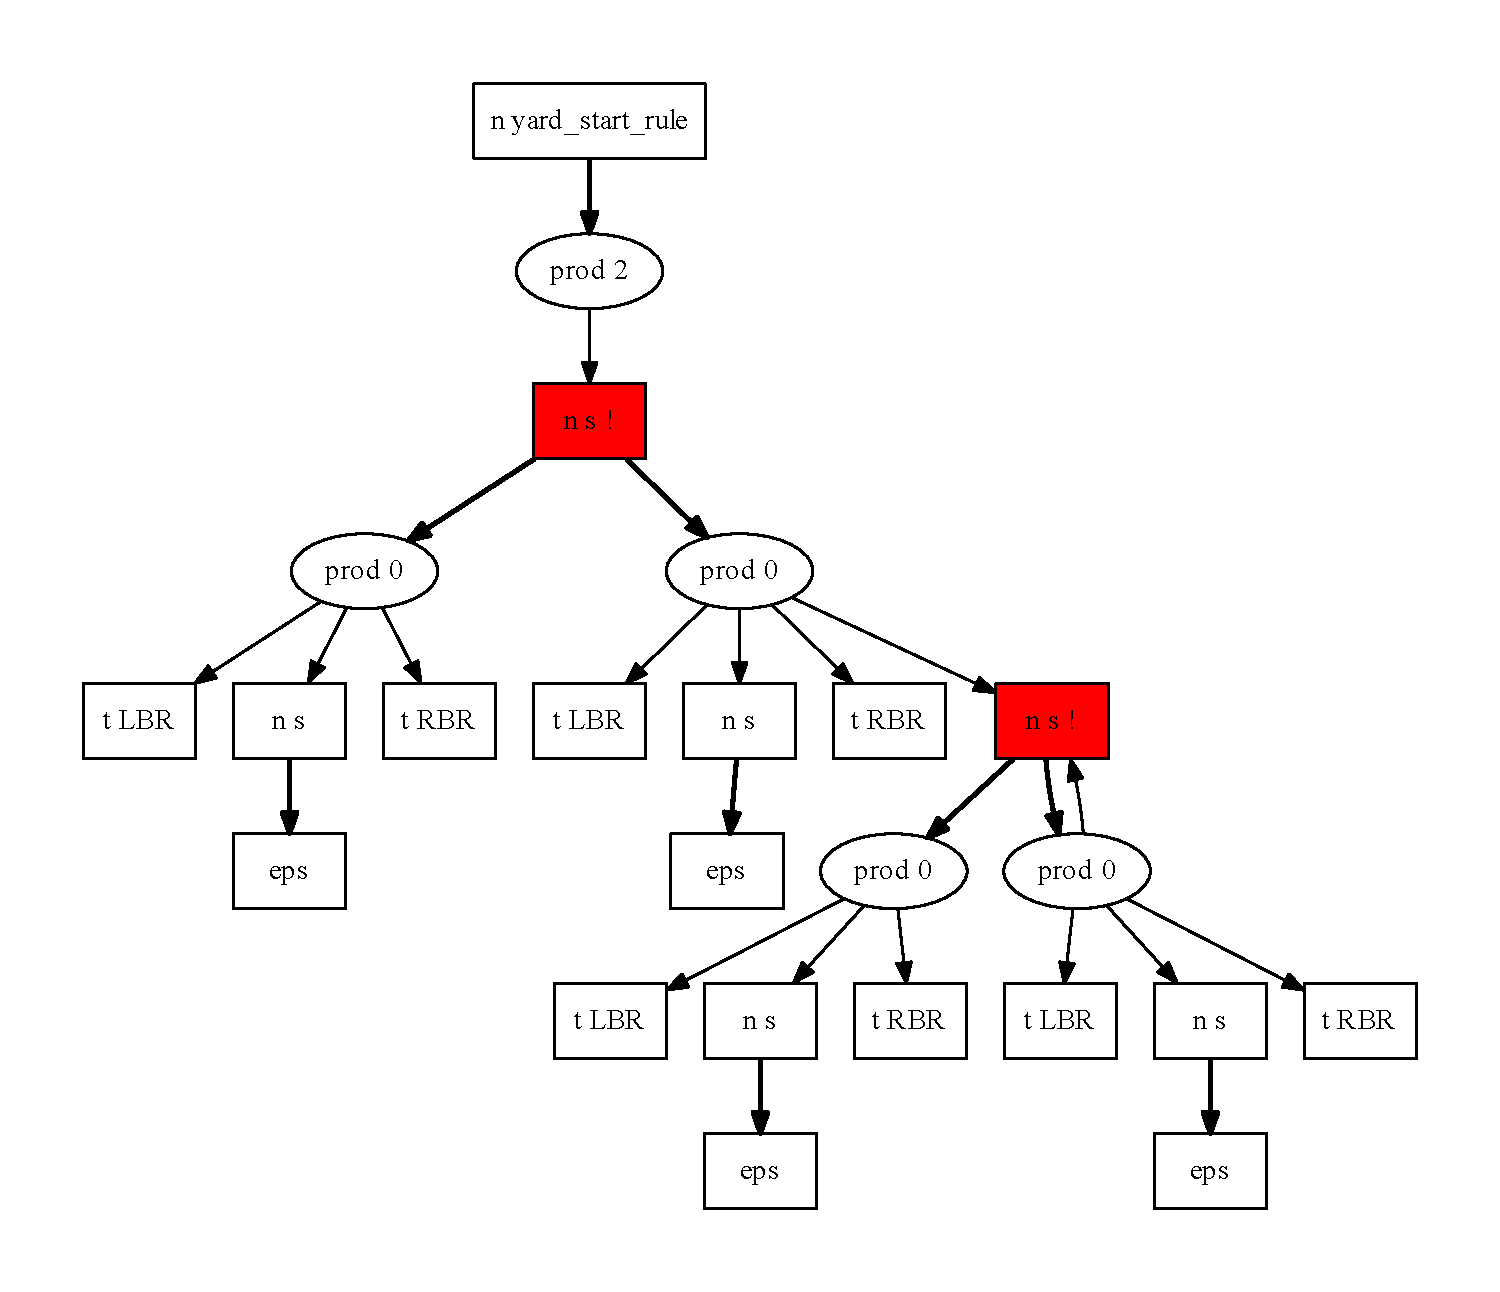
\includegraphics[width=6.8cm]{pictures/out3.pdf}}
\\
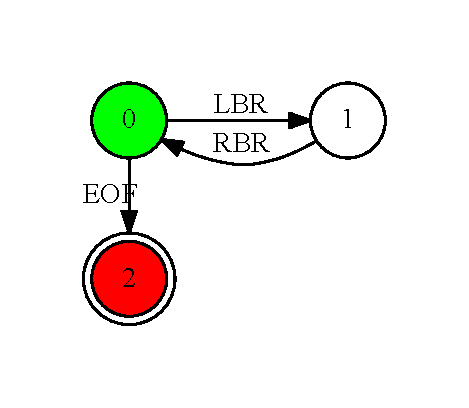
\includegraphics[width=2.5cm]{pictures/in3.pdf}
&
\\
Грамматика: &
\\
\vspace{-20pt}
% Можно формулы писать
{\begin{align*}
  start& & &\Coloneq & &s \\
  s & & &\Coloneq & &\mbox{\texttt{LBR }} s \mbox{\texttt{ RBR }} s \\
  s & & &\Coloneq & &\epsilon
\end{align*}}
&
\end{tabular}
\end{frame}


\begin{frame}
  \frametitle{Доказательство корректности алгоритма}
  {\tiny Формулировки утверждений. Идеи доказательств проговариваются устно.}
  \begin{rutheorem}[Пифагора: геометрическая формулировка]
    В прямоугольном треугольнике площадь квадрата, построенного на гипотенузе, равна сумме площадей квадратов, построенных на катетах.
  \end{rutheorem}

  \begin{rutheorem}[Пифагора: алгебраическая формулировка]
    В прямоугольном треугольнике квадрат длины гипотенузы равен сумме квадратов длин катетов.

    То есть, если обозначить длину гипотенузы треугольника через $c$, а длины катетов
через $a$ и $b$, получим верное равенство: $a^2 + b^2 = c^2$.
  \end{rutheorem}

  \begin{rutheorem}[Обратная теорема Пифагора]
    Для всякой тройки положительных чисел $a$, $b$ и $c$, такой, что $a^2 + b^2 = c^2$, существует прямоугольный треугольник с катетами $a$ и $b$ и гипотенузой $c$.
  \end{rutheorem}
\end{frame}

\begin{frame}
  \frametitle{Архитектура решения}
  \begin{itemize}
    \item В реализации интересны архитектура, библиотеки, инструменты
    \item Не надо добавлять на слайд примеры кода
  \end{itemize}
  \begin{center}
  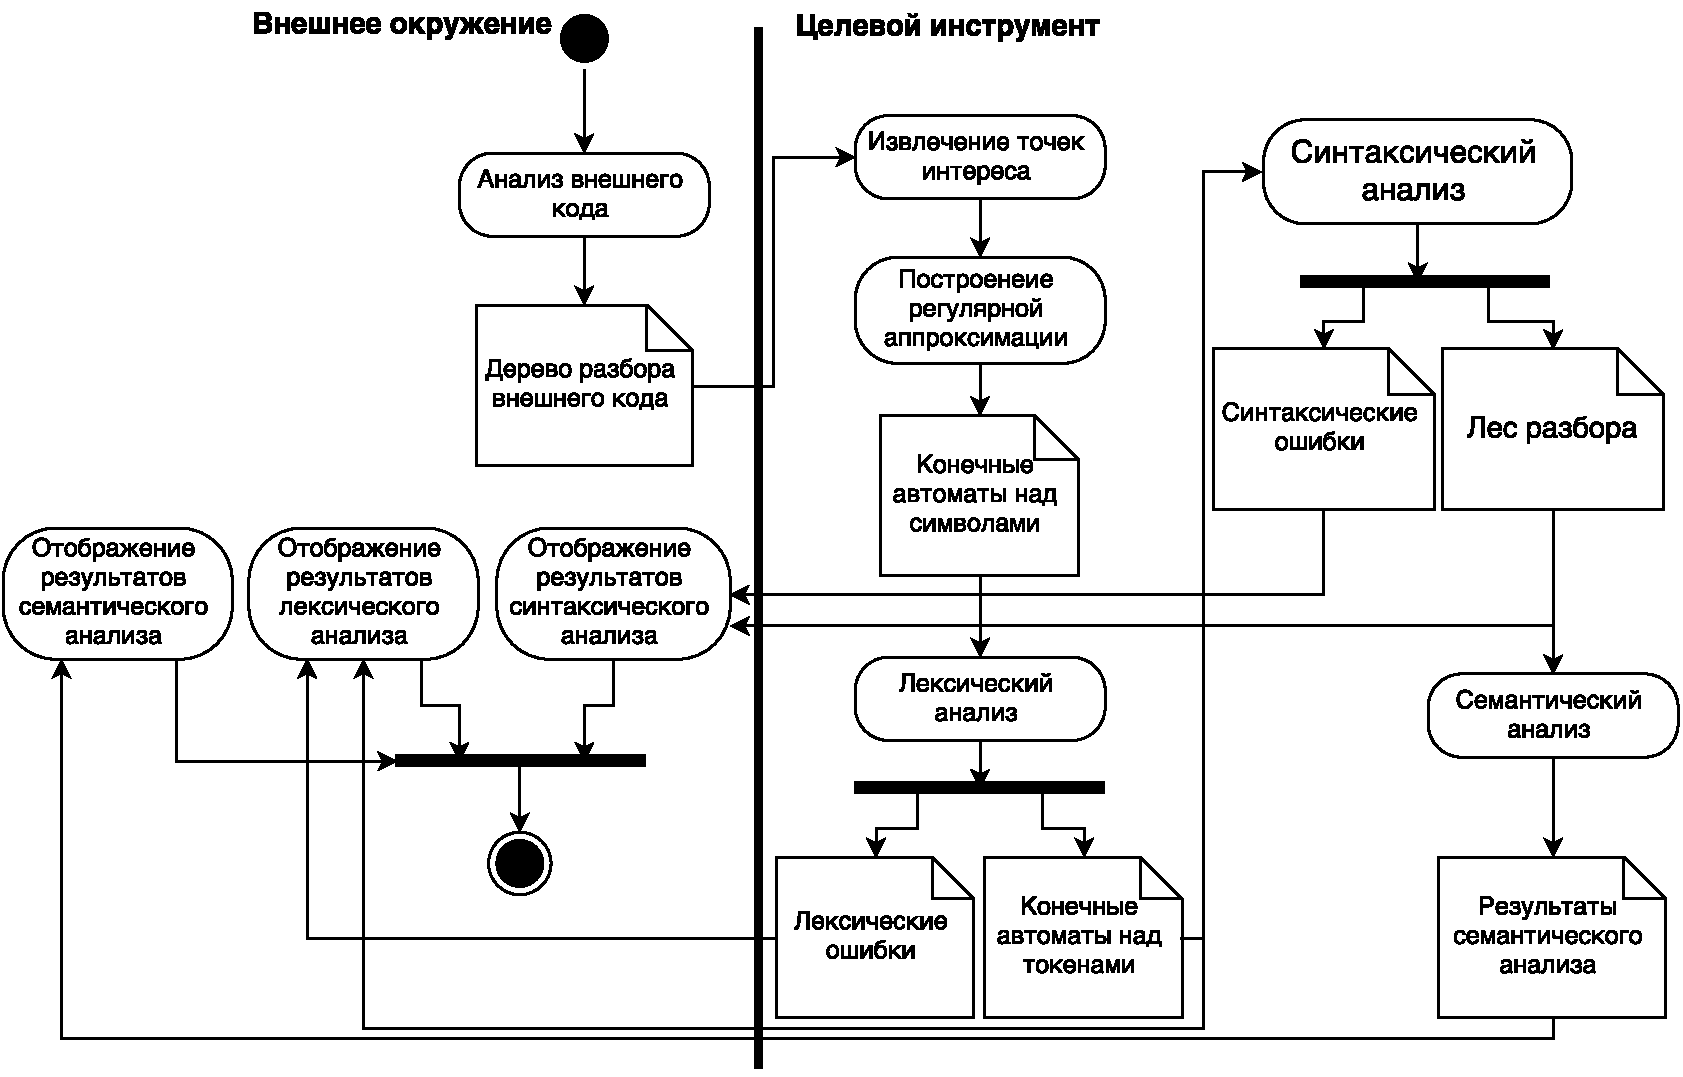
\includegraphics[width=0.8\textwidth]{pictures/Activ_SEL_Processing.pdf}
  \end{center}
\end{frame}

\begin{frame}[t]
  \frametitle{Экспериментальное исследование}
  Постановка эксперимента
  \begin{itemize}
    \item На каком наборе данных проводилось экспериментальное исследование, почему были выбраны именно эти данные
    \item На каком оборудовании проводилось исследование
    \item Какие решения были выбраны для сравнения и почему
  \end{itemize}
\end{frame}

\begin{frame}[t]
  \frametitle{Результаты экспериментального исследования}
  \begin{itemize}
    \item Какие результаты показало экспериментальное исследование
    \item Желательно привести графики, иллюстрирующие полученные результаты
    \begin{itemize}
      \item У иллюстраций должны быть подписи, у графиков~--- легенда, подписи к осям, например:
    \end{itemize}
  \end{itemize}
  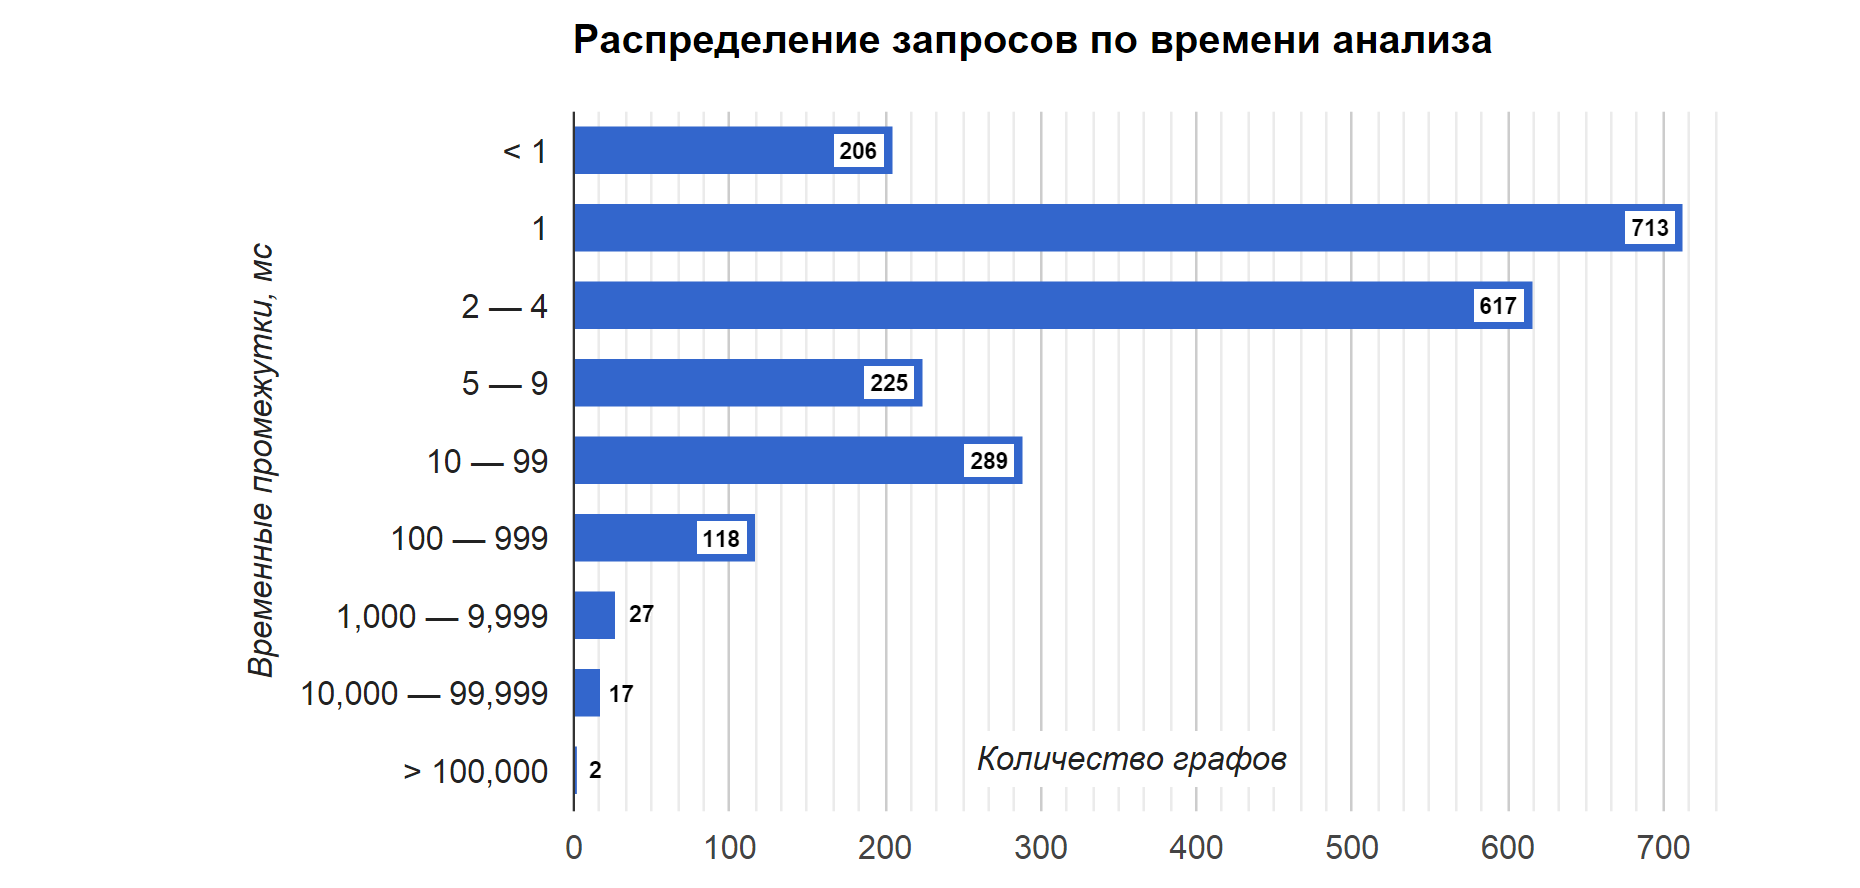
\includegraphics[width=10cm]{pictures/dist.png}
\end{frame}


\begin{frame}
  \frametitle{Результаты}
  \begin{itemize}
    \item Практически то же, что и на слайде с постановкой задачи, но в совершенной форме~--- что делал лично автор
    \item Четкое отделение результатов своей работы (особенно для коллективных работ)
      \item Формулировать глаголами совершенного вида в прошедшем времени (\enquote{сделано}, \enquote{получено})
    \item Обсуждение (ограничения, валидность, альтернативы)
    \item Не нужно слайдов типа \enquote{Все}, \enquote{Вопросы?}, \enquote{Спасибо за внимание}
  \end{itemize}

  \begin{itemize}
    \item Если результаты были представлены на конференции и опубликованы, это желательно указать
  \end{itemize}
\end{frame}

%\addtocounter{framenumber}{1}
\appendix

\begin{frame}
  \frametitle{Дополнительный слайд}
  Например, с огромной страшной формулой всего, которая нужна для пояснения деталей при ответе на частый вопрос

\begin{align*}
  \MoveEqLeft \lim_{\bigtriangleup t \to 0^+}\int_{\bigtriangleup t}^{T} \! \int_{\Omega} \! D(t_1,x) \frac{\varphi(t_1-\bigtriangleup t,x)-\varphi(t_1,x)}{(-\bigtriangleup t)} \, \mathrm{d}x \, \mathrm{d}t_1 \\
  &= \lim_{\bigtriangleup t \to 0^+} \int_{0}^{T} \! \int_{\Omega} \! D(t_1,x) \frac{\varphi(t_1-\bigtriangleup t,x)-\varphi(t_1,x)}{(-\bigtriangleup t)} \chi_{(\bigtriangleup t,T)}(t_1) \, \mathrm{d}x \, \mathrm{d}t_1 \\
  &=\int_{0}^{T} \! \int_{\Omega} \! D(t_1,x) \frac{\partial \varphi}{\partial t_1} (t_1,x) \, \mathrm{d}x \, \mathrm{d}t_1 .
\end{align*}
\end{frame}

\begin{frame}
  \frametitle{Второй дополнительный слайд}
\begin{itemize}
  \item Много дополнительных слайдов не надо: 1--2 вполне достаточно в большинстве случаев
  \item Кроме формул здесь могут быть схемы, рисунки, таблицы и другие вспомогательные материалы
\end{itemize}


\end{frame}

\end{document}